\label{sec:clusters}
In this section we try to compare the performance of RMSD task on different HPC resources to examine the robustness of the methods we used for our performance study.
HPC resources used for this purpose and their system configuration are given in Table \ref{tab:sys-config}.
We perform these comparisons for several cases discussed previously. 
These cases include: Splitting the trajectories with collective communications in MPI, Splitting the trajectories with global array for communications, and MPI-based Parallel HDF5.

\subsection{Splitting the Trajectories}
Figure \ref{fig:MPI-splitting-clusters} shows how RMSD task scales with the increase in the number of cores on different HPC resources.  
When we split the trajectories the scaling follows the same pattern on both Comet and SuperMIC with global array and without global array.
Both Comet and SuperMIC scales very well using Global array. 
RMSD task still scales on both clusters without global array; however, scaling is far from ideal scaling due to the communication cost (Refer to section \ref{Splitting} and Figure \ref{fig:MPIranks-split}). 
Overal, the scaling of the RMSD task is better on SuperMIC and the performance gap increases as we increase the number of cores.
This is expected for the following reasons:
First, CPU speed on SuperMIC is 2.8 GHz vs 2.5 GHz on Comet. This is $\approx 12\%$ performance difference in favor of SuperMIC\gpnote{This type of comparing may have been correct assuming you used only 20 cores on Comet, 10 from each processor. But all of them were used, right?}. \mknote{Yes, all the cores are used but I do not understand why you say when all core numbers are used this type of comparison is not correct.}
Second, for the same network speed the number of cores per node on SuperMIC (20 cores per node) is smaller than Comet (24 cores per node). 
Therefore, access to memory per core should be factor of $12/10 \approx 20\%$ faster on SuperMIC\gpnote{Memory access performance is not measured be the number of cores accessing the memory only. First, SuperMic has DDR3, and Comet has DDR4. Just that shows us that Comet memory is better. We do not have data as memory read/write times, memory organization and architecture, that is every memory address how many data can it hold? Any information on memory throughput? I would never do this type of arithmetic to compare CPUs and memory.}\mknote{I agree with you. But do you have any suggestion on how we should discuss these differences?}
\gpnote{Also, I am not sure whether GA support direct memory access from the network card or not. If you have a reference that says so, please cite it here, otherwise I would remove the argument}.
\mknote{What is direct memory access from the network card? Why does it matter?}

\begin{figure}[ht!]
\centering
\begin{subfigure}{.4\textwidth}
  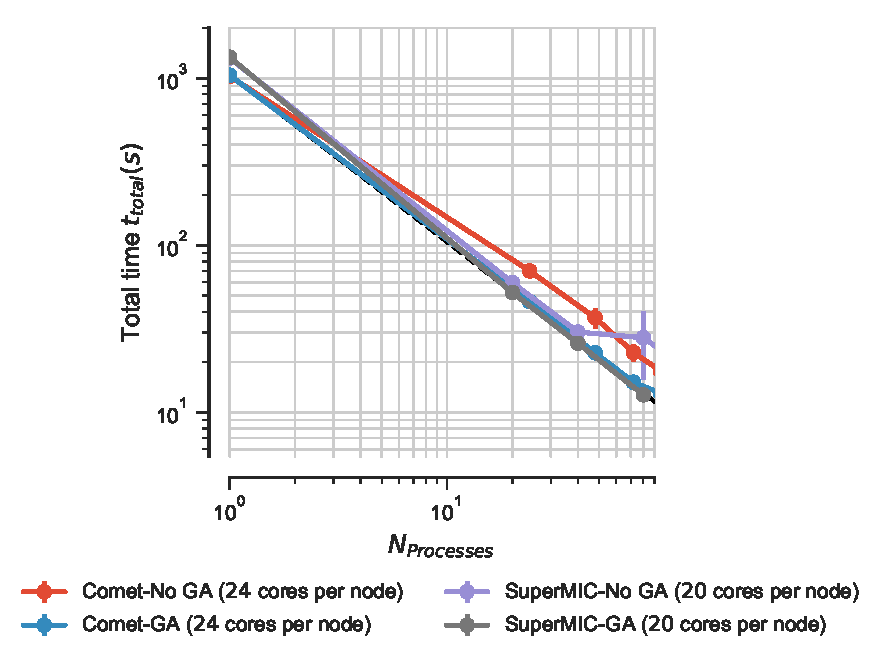
\includegraphics[width=\linewidth]{figures/Comparison_t-tot-clusters_Splitting.pdf}
  \caption{Scaling total}
  \label{fig:MPIscaling-clusters-splitting}
\end{subfigure}
\hfill
\begin{subfigure}{.4\textwidth}
  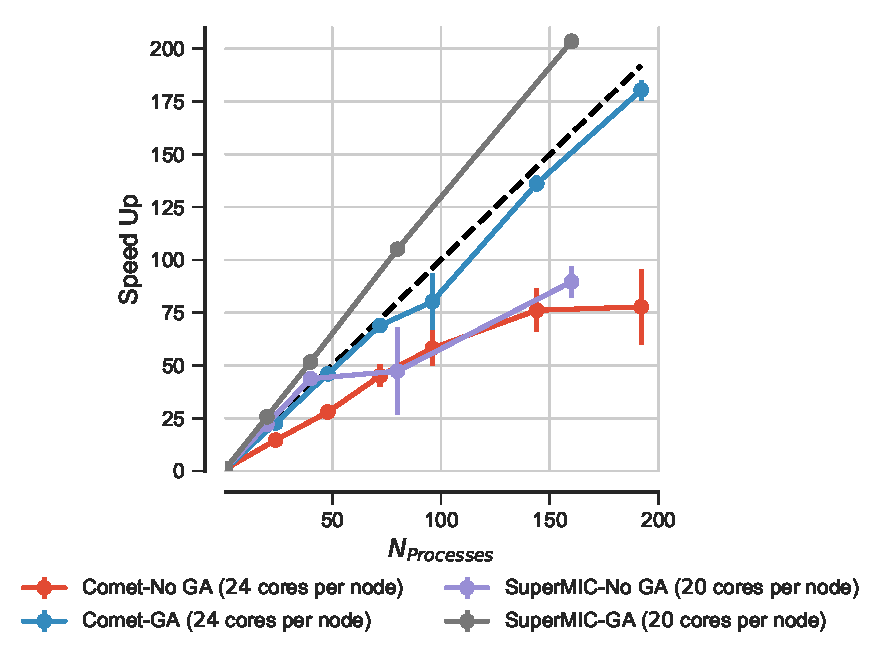
\includegraphics[width=\linewidth]{figures/Comparison_speed-up-clusters_Splitting.pdf}
  \caption{Speed-up}
  \label{fig:MPIspeedup-clusters-splitting}
\end{subfigure}
\bigskip

\begin{subfigure} {.8\textwidth}
  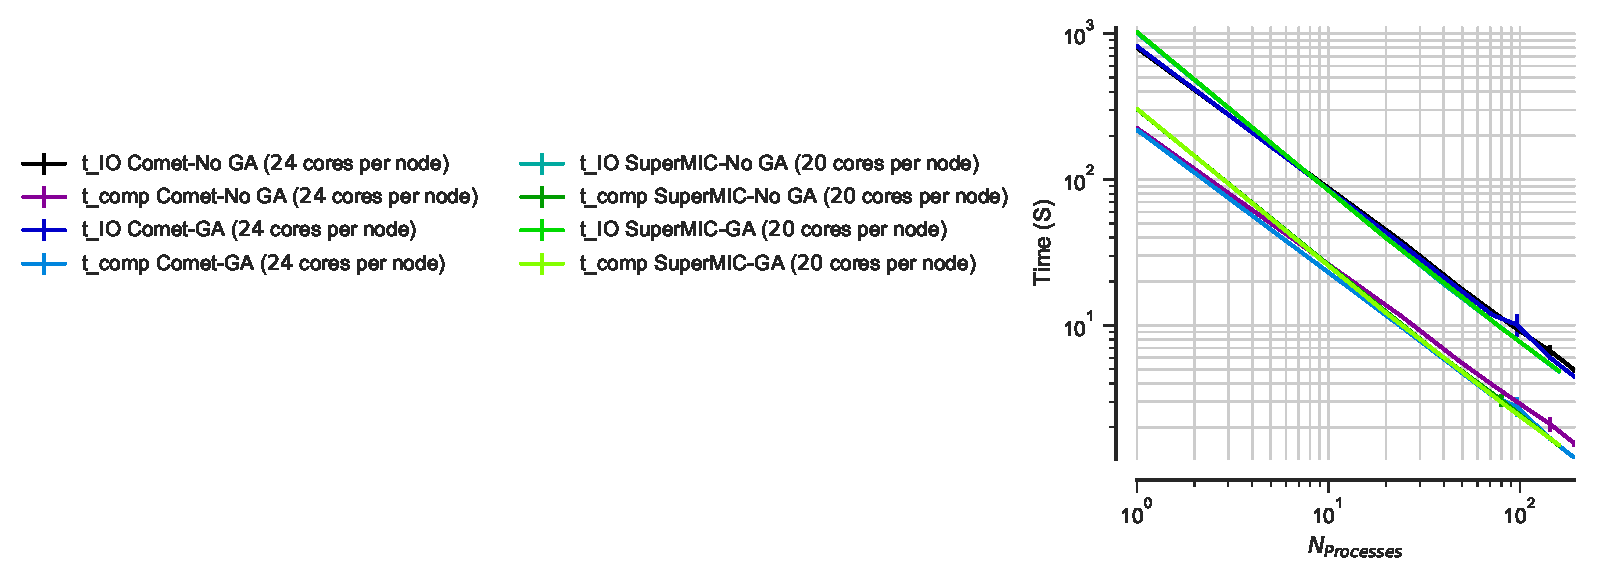
\includegraphics[width=\linewidth]{figures/Clusters_IO_compute_scaling_splitting.pdf}
  \caption{Scaling of the \tcomp and \tIO of the RMSD task with MPI when the trajectories are splitted using global array and without global array.}
  \label{fig:compute-IO-scaling-clusters-splitting}
\end{subfigure}
%
\caption{Comparison of the performance of the RMSD task with MPI ($\tcomp/\tIO \approx 0.3$) when the trajectories are splitted using global 
array and without global array across different clusters (SDSC Comet, SuperMIC). Data are read from the file system (I/O included).
In case of global array, all ranks update the global array ($ga_{put}$) and rank 0 accesses the whole RMSD array through the global memory address ($ga_{get}$).
Five repeats are performed to collect statistics. The error bars show standard deviation with respect to mean. }
\label{fig:MPI-splitting-clusters}
\end{figure} 

\subsection{MPI-based Parallel HDF5}
\gpnote{Same as above}
Figure \ref{fig:MPIwithIO-clusters} shows how RMSD task scales with the increase in the number of cores on different HPC resources using MPI-based parallel HDF5.  
The scaling follows the same pattern on both Comet and SuperMIC. 
Both Comet and SuperMIC scales very well.
Overal, the scaling of the RMSD task is better on SuperMIC for the reasons that discussed above.
Bridge performance is different from Comet and SuperMIC.
Bridge has 28 cores per compute node and when we use all cores for our calculations there is no scaling.
However, decreasing the number of cores per node and having uniform workload distributions across all nodes can lead to significant improvements in the scaling as shown in Figure \ref{fig:MPIwithIO-clusters}.
The reason for performance difference between Comet and Bridges can be explained as below:
First, CPU speed on Bridges is 2.3 GHz vs 2.5 GHz on Comet. This is $\approx 8.6\%$ performance difference in favor of Comet. 
Second, for the same network speed the number of cores per node on Bridge (28 cores per node) is larger than Comet (24 cores per node). 
Therefore, access to memory per core should be factor of $14/12 \approx 16\%$ faster on Comet.
The memory access effect on the timing distribution across different rank is shown for one run of the 5 repeats (Figure \ref{fig:MPIwithIO-clusters-rank}).
Based on Figure \ref{fig:MPIwithIO-clusters-rank} the I/O time distribution is pretty small and uniform across all ranks on Comet and SuperMIC (Figures \ref{fig:hdf5-SuperMIC} \& \ref{fig:MPIranks-hdf5}).
However, on Bridges the I/O time is on average about two and a half times larger and the I/O time distribution is also erratic across different ranks (Figure \ref{fig:hdf5-bridge}).  

\begin{figure}[ht!]
\centering
\begin{subfigure}{.4\textwidth}
  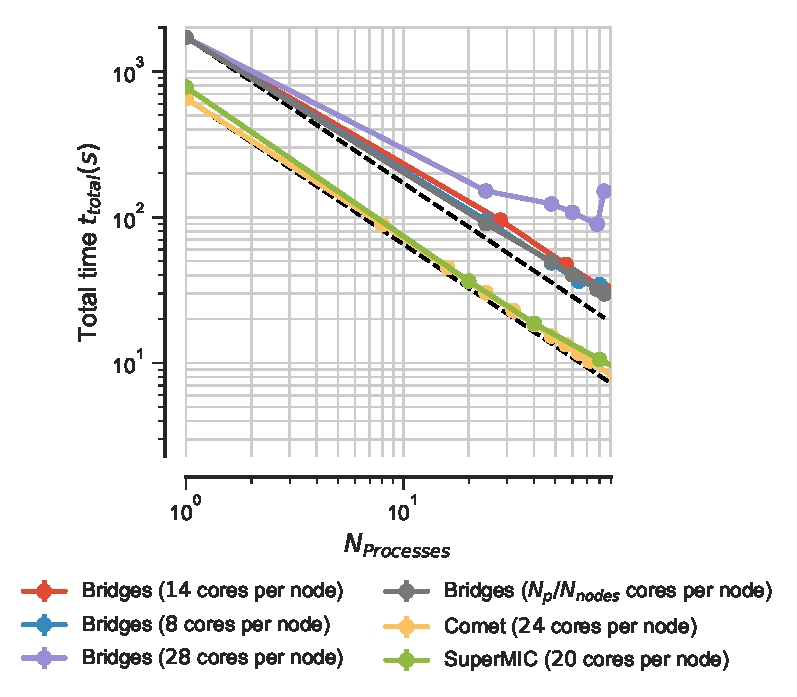
\includegraphics[width=\linewidth]{figures/Comparison_t-tot-clusters.pdf}
  \caption{Scaling total}
  \label{fig:MPIscaling-clusters}
\end{subfigure}
\hfill
\begin{subfigure}{.4\textwidth}
  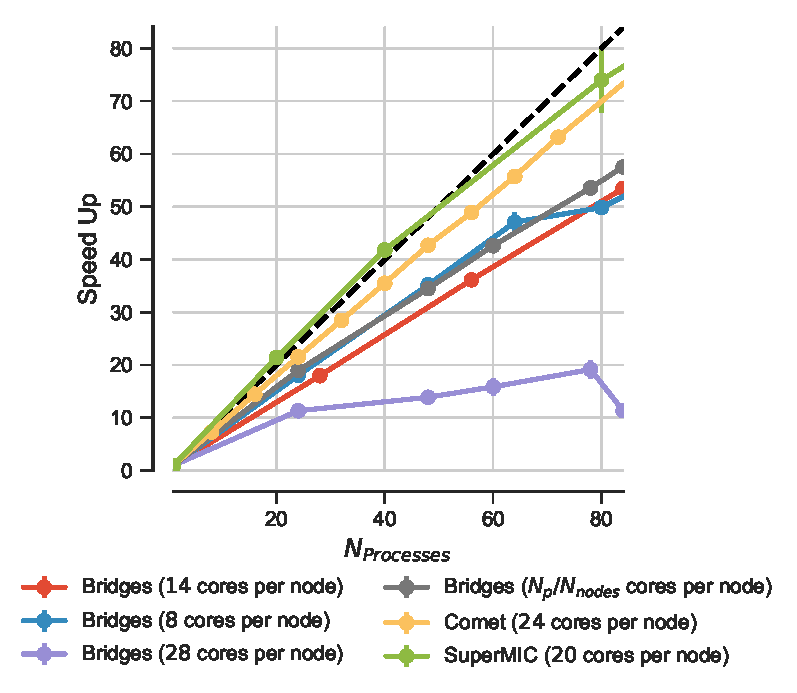
\includegraphics[width=\linewidth]{figures/Comparison_speed-up-clusters.pdf}
  \caption{Speed-up}
  \label{fig:MPIspeedup-clusters}
\end{subfigure}
\bigskip

\begin{subfigure} {.8\textwidth}
  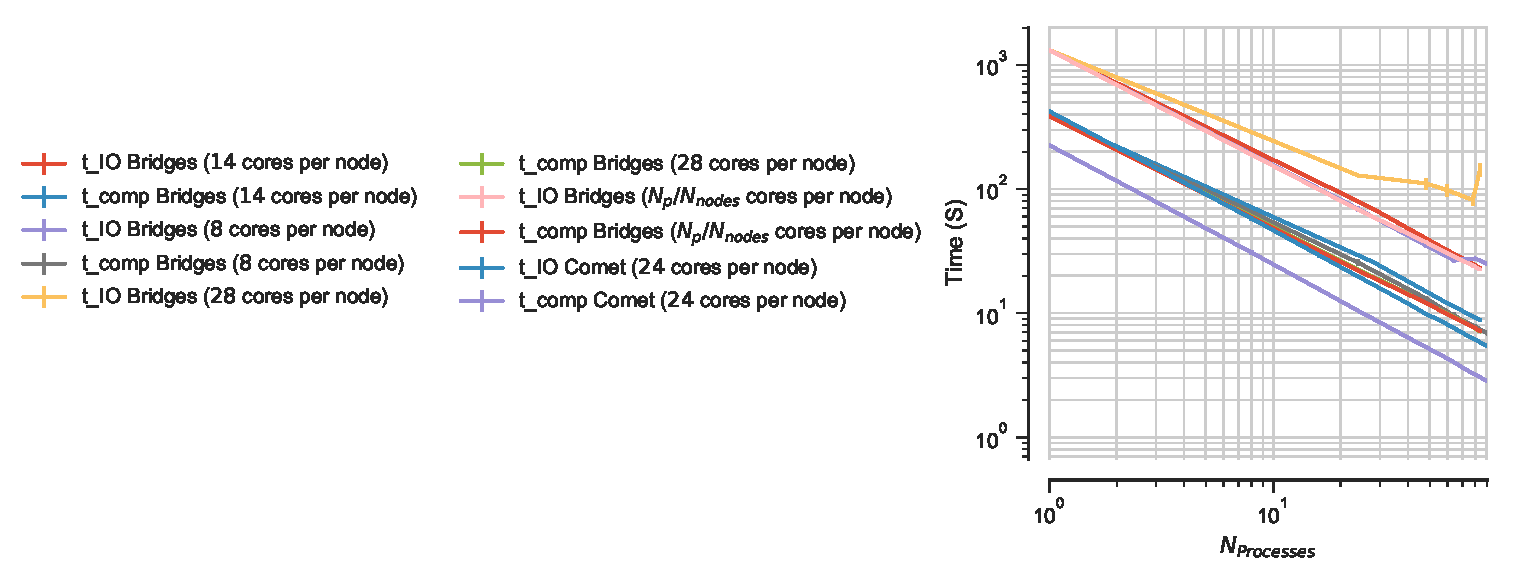
\includegraphics[width=\linewidth]{figures/Clusters_IO_compute_scaling.pdf}
  \caption{Scaling of the \tcomp and \tIO of the RMSD task with MPI-based parallel HDF5 (Independent I/O)}
  \label{fig:compute-IO-scaling-clusters}
\end{subfigure}
%
\caption{Comparison of the performance of the RMSD task with MPI ($\tcomp/\tIO \approx 0.3$)
across different clusters (SDSC Comet, PSC Bridge, SuperMIC). Data are read from a shared HDF5 file format instead of XTC format (Independent I/O)
and results are communicated back to rank 0 (communications included). Five repeats are performed to 
collect statistics. The error bars show standard deviation with respect to mean.}
\label{fig:MPIwithIO-clusters}
\end{figure} 

\begin{figure}[ht!]
\centering
\begin{subfigure}{.45\textwidth}
  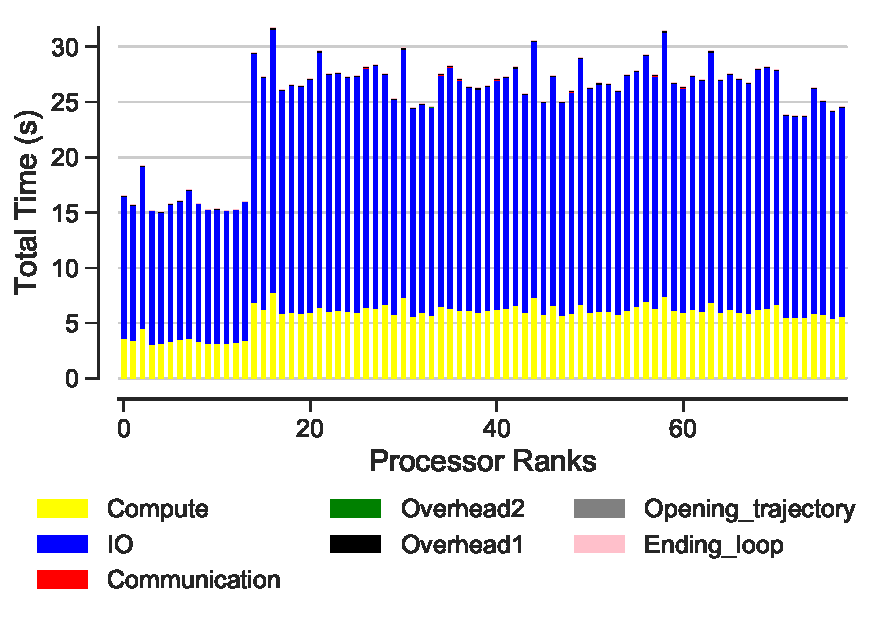
\includegraphics[width=\linewidth]{figures/Bridge-MPI-IO-BarPlot-rank-comparison_78_5.pdf}
  \caption{Bridge}
  \label{fig:hdf5-bridge}
\end{subfigure}
\bigskip
\begin{subfigure} {.45\textwidth}
  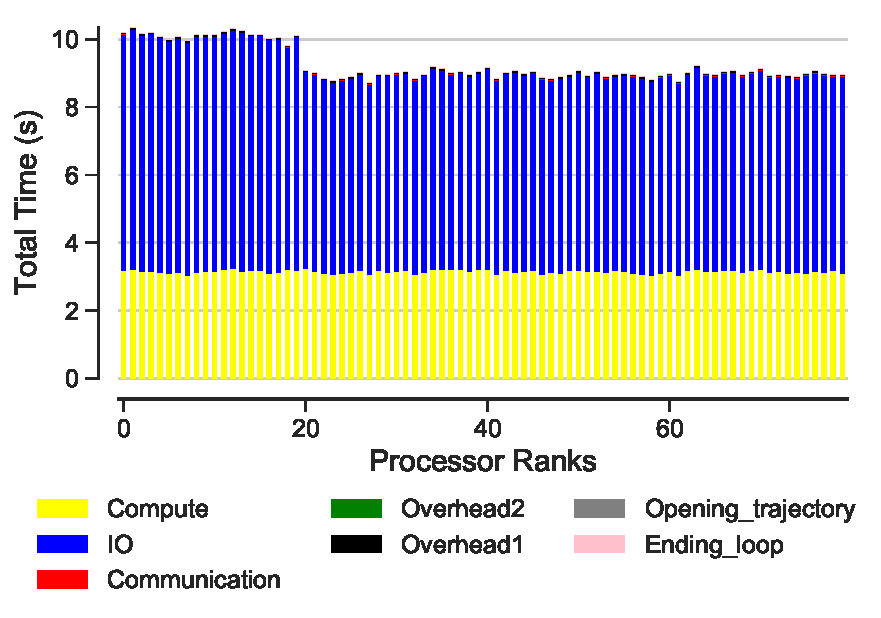
\includegraphics[width=\linewidth]{figures/SuperMIC-MPI-IO-BarPlot-rank-comparison_80_5.pdf}
  \caption{SuperMIC}
  \label{fig:hdf5-SuperMIC}
\end{subfigure}
%
\caption{Examples of timing per MPI rank for RMSD task with MPI-based parallel HDF5 ($\tcomp/\tIO \approx 0.3$) on (a) PSC Bridge and (b) SuperMIC (Buttomn).
Five repeats are performed to collect statistics and this is typical data from one run of the 5 repeats. Compute \tcomp, IO \tIO, communication \tcomm, ending the for loop $t_{end\_loop}$,
opening the trajectory $t_{opening\_trajectory}$, and overheads $t_{Overhead1}$,  $t_{Overhead2}$ per MPI rank (as described in methods).
This is typical data from one run of the 5 repeats. I/O distribution is non-uniform on Bridge while it is more uniform on SuperMIC and this explains why SuperMIC has better scaling as compared to PSC Bridge.}
\label{fig:MPIwithIO-clusters-rank}
\end{figure} 

\subsection{Comparison of Compute \& I/O Scaling Across Different Clusters}
Comparison of compute \& I/O scaling across different clusters for different test cases and algorithms is shown in Table \ref{tab:comp-IO-scaling}. 
The corresponding plots for compute and I/O scaling are shown in related sections. 
These plots together with Table \ref{tab:comp-IO-scaling} allow both quantitative and qualitative comparison of the compute and I/O time scaling.
As can be seen in Table \ref{tab:comp-IO-scaling} for MPI-based parallel HDF5, both compute and I/O time on Bridge is larger than its corresponding value on Comet and SuperMIC.
For example, with one core the corresponding compute and I/O time are about (387, 1318) versus (225, 423) and (273, 503) on Comet and SuperMIC respectively.
This performance difference becomes more obvious as the number of cores increases.
When the trajectories are splitted and global array is used for communication both Comet and SuperMIC show similar performance at small number of cores and the their performance difference increases as the number of cores increases. 
The reason why we see these performance differences is explained in previous sections. 

\begin{sidewaystable}[ht!]
\centering
\begin{adjustbox}{max width=\textwidth}
\begin{tabular}{c c c c c c c c c c c c c c}
  \toprule
 \multicolumn{10}{r}{\bfseries $N_{Processes}$} \\
\cmidrule(r){7-14}
           \bfseries\thead{Cluster} & \bfseries\thead{Calculation} & \bfseries\thead{Load Ratio} & \bfseries\thead{Gather} & \bfseries\thead{File Access} & \bfseries\thead{Time} & \bfseries\thead{1} & \begin{tabular}{c} \bfseries\thead{Comet:} 24 \\ \bfseries\thead{Bridges:} 24 \\ \bfseries\thead{SuperMIC:} 20 \end{tabular}  & \begin{tabular}{c} \bfseries\thead{Others:} 48 \\ \bfseries\thead{Bridges:} 48 \\ \bfseries\thead{SuperMIC:} 40 \end{tabular} & \begin{tabular}{c} \bfseries\thead{Comet:} 72 \\ \bfseries\thead{Bridges:} 60 \\ \bfseries\thead{SuperMIC:} 80 \end{tabular} & \begin{tabular}{c} \bfseries\thead{Comet:} 96 \\ \bfseries\thead{Bridges:} 78 \end{tabular} & \begin{tabular}{c} \bfseries\thead{Comet:} 144 \\ \bfseries\thead{Bridges:} 84 \\ \bfseries\thead{SuperMIC:} 160\end{tabular} & \bfseries\thead{Comet: 192} & \begin{tabular}{c} \bfseries\thead{Comet:} 384 \\  \bfseries\thead{SuperMIC:} 320\end{tabular}\\
  \midrule
   Comet & \makecell{Dihedral \\Featurization} & 100 & MPI & Single & \begin{tabular}{c} \tIO \\ \tcomp \end{tabular} & \begin{tabular}{c} $2880 \pm 0$ \\ $272000 \pm 0$ \end{tabular} & \begin{tabular}{c} $40 \pm 1.63$ \\ $12440 \pm 200.78$ \end{tabular} & \begin{tabular}{c} $20 \pm 1.22$ \\ $6305 \pm 38.13$ \end{tabular} & \begin{tabular}{c} $15 \pm 3.91$ \\ $4225 \pm 83.41$ \end{tabular} & -- & -- & --& --\\ 
  \midrule
    Comet & RMSD 1X & 0.3 & MPI & Single & \begin{tabular}{c} \tIO \\ \tcomp  \end{tabular} & \begin{tabular}{c} $799 \pm 5.22$ \\ $225 \pm 5.4$ \end{tabular} & \begin{tabular}{c} $49 \pm 3.45$ \\ $11 \pm 0.75$ \end{tabular} & \begin{tabular}{c} $29 \pm 1.3$ \\ $6 \pm 0.35$ \end{tabular} & \begin{tabular}{c} $26 \pm 9.19$ \\ $4 \pm 0.48$ \end{tabular} & -- & -- & -- & --\\  
  \midrule
    Comet & RMSD 1X & 0.3 & GA & Single & \begin{tabular}{c} \tIO \\ \tcomp \end{tabular} & \begin{tabular}{c} $820 \pm 18.49$ \\ $219 \pm 9.8$ \end{tabular} & \begin{tabular}{c} $41 \pm 8.99$ \\ $10 \pm 0.3$ \end{tabular} & \begin{tabular}{c} $23 \pm 4.14$ \\ $5 \pm 0.48$ \end{tabular} & \begin{tabular}{c} $15 \pm 2.06$ \\ $3 \pm 0.54$ \end{tabular} & -- & -- & -- & --\\
  \midrule
    Comet & RMSD 1X & 0.3 & MPI & Splitting & \begin{tabular}{c} \tIO \\ \tcomp \end{tabular} & \begin{tabular}{c} $799 \pm 5.22$ \\ $225 \pm 5.4$ \end{tabular} & \begin{tabular}{c} $37 \pm 1.22$ \\ $11 \pm 0.31$ \end{tabular} & \begin{tabular}{c} $18 \pm 0.18$ \\ $5 \pm 0.07$ \end{tabular} & \begin{tabular}{c} $12 \pm 0.14$ \\ $3 \pm 0.04$ \end{tabular} & \begin{tabular}{c} $9 \pm 0.3$ \\ $3 \pm 0.11$ \end{tabular} & \begin{tabular}{c} $6  \pm 0.66$ \\ $2 \pm 0.23$ \end{tabular} & \begin{tabular}{c} $4 \pm 0.23$ \\ $1 \pm 0.07$ \end{tabular} & --\\
  \midrule
    SuperMIC & RMSD 1X & 0.3 & MPI & Splitting & \begin{tabular}{c} \tIO \\ \tcomp \end{tabular} & \begin{tabular}{c} $1013.75 \pm 2.8$ \\ $304.26 \pm 2.55$ \end{tabular} & \begin{tabular}{c} $39.99 \pm 0.36$ \\ $12.41 \pm 0.22$ \end{tabular} & \begin{tabular}{c} $19.18 \pm 0.25$ \\ $5.99\pm 0.09$ \end{tabular} & \begin{tabular}{c} $9.61 \pm 0.28$ \\ $3.08 \pm 0.13$ \end{tabular} & -- & \begin{tabular}{c} $4.83 \pm 0.06$ \\ $1.5 \pm 0.01$ \end{tabular} & --& --\\ 
  \midrule 
    Comet & RMSD 1X & 0.3 & GA & Splitting & \begin{tabular}{c} \tIO \\ \tcomp \end{tabular} & \begin{tabular}{c} $820 \pm 18.5$ \\ $219 \pm 9.5$ \end{tabular} & \begin{tabular}{c} $36 \pm 0.78$ \\ $9 \pm 0.22$ \end{tabular} & \begin{tabular}{c} $17 \pm 0.3$ \\ $4 \pm 0.07$ \end{tabular} & \begin{tabular}{c} $11 \pm 0.23$ \\ $3 \pm 0.04$ \end{tabular} & \begin{tabular}{c} $10 \pm 1.7$ \\ $2 \pm 0.4$ \end{tabular} & \begin{tabular}{c} $5 \pm 0.14$ \\ $1 \pm 0.05$ \end{tabular} & \begin{tabular}{c} $4 \pm 0.07$ \\ $1 \pm 0.02$ \end{tabular} & --\\
  \midrule
    SuperMIC & RMSD 1X & 0.3 & GA & Splitting & \begin{tabular}{c} \tIO \\ \tcomp \end{tabular} & \begin{tabular}{c} $1027.62 \pm 10.32$ \\ $305.78 \pm 3.47$ \end{tabular} & \begin{tabular}{c} $39.62 \pm 0.2$ \\ $12.16 \pm 0.1$ \end{tabular} & \begin{tabular}{c} $19.66 \pm 0.1$ \\ $6.01\pm 0.007$ \end{tabular} & \begin{tabular}{c} $9.57 \pm 0.1$ \\ $2.97 \pm 0.1$ \end{tabular} & -- & \begin{tabular}{c} $4.86 \pm 0.05$ \\ $1.51 \pm 0.03$ \end{tabular} & --& --\\     
  \midrule
    Comet & RMSD 1X & 0.3 & MPI & PHDF5 & \begin{tabular}{c} \tIO \\ \tcomp \end{tabular} & \begin{tabular}{c} $423 \pm 5.88$ \\ $225 \pm 6.55$ \end{tabular} & \begin{tabular}{c} $19 \pm 0.3$ \\ $10 \pm 0.12$ \end{tabular} & \begin{tabular}{c} $9 \pm 0.13$ \\ $5 \pm 0.1$ \end{tabular} & \begin{tabular}{c} $6 \pm 0.06$ \\ $3 \pm 0.04$ \end{tabular} & \begin{tabular}{c} $5 \pm 0.12$ \\ $2 \pm 0.05$ \end{tabular} & \begin{tabular}{c} $3 \pm 0.2$ \\ $1 \pm 0.04$ \end{tabular} & \begin{tabular}{c} $3 \pm 0.25$\\ $1 \pm 0.03$ \end{tabular} & \begin{tabular}{c} $1.57 \pm 0.29$\\ $0.76 \pm 0.09$ \end{tabular}\\
  \midrule 
    Bridges & RMSD 1X & 0.3 & MPI & PHDF5 & \begin{tabular}{c} \tIO \\ \tcomp \end{tabular} & \begin{tabular}{c} $1318.87 \pm 10.42$ \\ $387.8 \pm 5.51$ \end{tabular} & \begin{tabular}{c} $67.93 \pm 0.52$ \\ $21.97 \pm 0.38$ \end{tabular} & \begin{tabular}{c} $37.37 \pm 0.2$ \\ $12.12 \pm 0.34$ \end{tabular} & \begin{tabular}{c} $30.35 \pm 0.15$ \\ $9.79 \pm 0.24$ \end{tabular} & \begin{tabular}{c} $24.16 \pm 0.89$ \\ $7.72 \pm 0.03$ \end{tabular} & \begin{tabular}{c} $22.5 \pm 0.17$ \\ $7.18 \pm 0.08$ \end{tabular} & -- & --\\ 
  \midrule
    SuperMIC & RMSD 1X & 0.3 & MPI & PHDF5 & \begin{tabular}{c} \tIO \\ \tcomp \end{tabular} & \begin{tabular}{c} $503.69 \pm 2.57$ \\ $273.54 \pm 4.7$ \end{tabular} & \begin{tabular}{c} $12.96 \pm 0.06$ \\ $23.44 \pm 0.29$ \end{tabular} & \begin{tabular}{c} $6.46 \pm 0.02$ \\ $12.22 \pm 0.43$ \end{tabular} & \begin{tabular}{c} $3.2 \pm 0.01$ \\ $7.3 \pm 0.85$ \end{tabular} & -- & \begin{tabular}{c} $1.64 \pm 0.01$ \\ $4.59 \pm 0.96$ \end{tabular} & --& \begin{tabular}{c} $0.82 \pm 0.004$ \\ $1.55 \pm 0.009$ \end{tabular} \\
  \bottomrule
\end{tabular}
\end{adjustbox}
\caption[Notation of our performance modeling]
{Comparison of the compute and I/O scaling for different test cases and number of processes. Five repeats are performed to collect statistics. The mean value and the
standard deviation with respect to mean are reported for each case.\gpnote{The font is extremely small in this table. Also can you add lines between different experiment configurations? Haven't the number of cores per node played a role to the overall performance?}\mknote{I corrected it. The number of cores per node has had effects and we need to have a discussion on that in text. Do you have any suggestion except from what I have disussed.}}
\label{tab:comp-IO-scaling}
\end{sidewaystable}

